\chapter{Casi d'uso}\label{CasiDUso}
In questo capitolo vengono elencati i casi d'uso$_G$ individuati per il progetto \textit{GDP: Gathering Detection Platform} in accordo con il proponente$_{\scaleto{G}{3pt}}$. Ogni caso d'uso$_{\scaleto{G}{3pt}}$ indica un'interazione tra uno o più attori e il sistema. Questa interazione genera uno scenario, cioè l'insieme delle azioni che hanno in comune uno scopo finale per un attore. I casi d'uso$_{\scaleto{G}{3pt}}$ vengono identificati nel seguente modo:
\begin{center}
	\textbf{UC[codice\_Padre].[codice\_Figlio]}
\end{center}
La descrizione della classificazione è la seguente:
\begin{itemize}
	\item \textbf{UC}: acronimo per User Case$_G$, parola inglese che si traduce in Casi D'uso$_{\scaleto{G}{3pt}}$;
	\item \textbf{Codice\_Padre.Codice\_Figlio}: codice univoco per ogni caso d'uso$_{\scaleto{G}{3pt}}$ nella forma gerarchica padre/figlio.
\end{itemize}

\section{Casi d'uso tra un utente e il front end}\label{CasiDUsoCasiDUsoTraUnUtenteEIlFrontEnd}
%spiegazione della sezione
\subsection{Attori dei casi d'uso}\label{CasiDUsoCasiDUsoTraUnUtenteEIlFrontEndAttoriDeiCasiDUso}
\begin{center}
	\begin{figure}[H]
		
\includegraphics{../immagini/attori_casi/utente_generico.png}
		\caption{Attore: utente generico}
	\end{figure}
\end{center}
\subsubsection{Attori Primari}\label{CasiDUsoCasiDUsoTraUnUtenteEIlFrontEndAttoriDeiCasiDUsoAttoriPrimari}
\begin{itemize}
	\item \textbf{Utente generico:} definisce l'utente generico che utilizza l'applicazione web;
\end{itemize}

\subsection{Elenco casi d'uso}\label{CasiDUsoCasiDUsoTraUnUtenteEIlFrontEndElencoCasiDUso}

\subsubsection{UC1 - Visualizzazione informazioni sulla mappa}\label{CasiDUsoCasiDUsoTraUnUtenteEIlFrontEndElencoCasiDUsoUC1VisualizzazioneInformazioniSullaMappa} %parzialmente corretto

\begin{center}
	\begin{figure}[H]
		\centering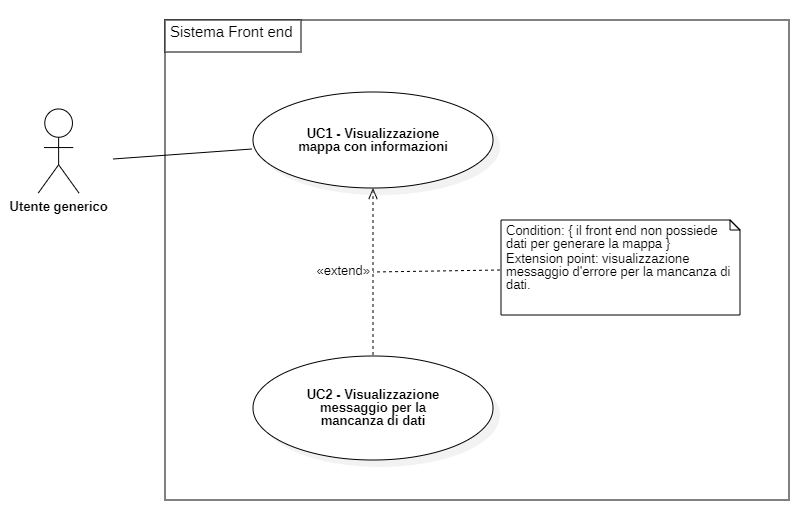
\includegraphics[scale=0.8]{../immagini/attori_casi/uc1_uc2.png}
		\caption{UC1 - Visualizzazione informazioni sulla mappa}
	\end{figure}
\end{center}

\begin{itemize}
	\item \textbf{Attori primari}: utente generico;
	\item \textbf{Descrizione}: l’utente accede all’applicazione web e visualizza la heat map$_{\scaleto{G}{3pt}}$. La mappa mostra la città impostata di default o quella selezionata tra quelle a disposizione, come definito nell’UC4(sezione \S~\ref{CasiDUsoCasiDUsoTraUnUtenteEIlFrontEndElencoCasiDUsoUC4SelezioneCittaDaVisualizzareNellaMappa}). Le informazioni vengono ricavate dall’orario e la data impostate dall’utente come indicato nel UC5.1(sezione \S~\ref{CasiDUsoCasiDUsoTraUnUtenteEIlFrontEndElencoCasiDUsoUC51SelezioneDellOrario}) e UC5.2(sezione \S~\ref{CasiDUsoCasiDUsoTraUnUtenteEIlFrontEndElencoCasiDUsoUC52ModificaDellaData}) o si utilizzano i dati in tempo reale quindi usando l’orario attuale;
	\item \textbf{Scenario principale}: L’utente accede all’applicazione web e visualizza la heat map$_{\scaleto{G}{3pt}}$ della città;
	\item \textbf{Precondizione}: il front end$_{\scaleto{G}{3pt}}$ può generare la mappa; la città, la data, l’ora sono state indicate dall’utente, seguendo quanto descritto rispettivamente nell'UC4 (sezione \S~\ref{CasiDUsoCasiDUsoTraUnUtenteEIlFrontEndElencoCasiDUsoUC4SelezioneCittaDaVisualizzareNellaMappa}), nell'UC5.2(sezione \S~\ref{CasiDUsoCasiDUsoTraUnUtenteEIlFrontEndElencoCasiDUsoUC52ModificaDellaData}) e nell'UC5.1(sezione \S~\ref{CasiDUsoCasiDUsoTraUnUtenteEIlFrontEndElencoCasiDUsoUC51SelezioneDellOrario}), o vengono utilizzate quelle di default, quindi data e ora sono quelle odierne di sistema per dati in tempo reale e la città è quella impostata di default;
	\item \textbf{Postcondizione}: l’utente visualizza la heat map$_{\scaleto{G}{3pt}}$ con i dati ricavati nell’istante di tempo selezionato, come definito nell’UC5 (sezione \S~\ref{CasiDUsoCasiDUsoTraUnUtenteEIlFrontEndElencoCasiDUsoUC5SelezioneDellIstanzeDiCuiVisualizzareIDatiNellaHeatmap}), e alla città scelta fra quelle disponibili come descritto nella definizione dell’UC4 (sezione \S~\ref{CasiDUsoCasiDUsoTraUnUtenteEIlFrontEndElencoCasiDUsoUC4SelezioneCittaDaVisualizzareNellaMappa});
	\item \textbf{Estensioni}: l’utente accede all’applicazione web, il front end$_{\scaleto{G}{3pt}}$, rilevando la richiesta di generazione della mappa, individua una mancanza di dati per la sua costruzione e di conseguenza viene visualizzato un messaggio relativo all’errore riscontrato (UC2, sezione \S~\ref{CasiDUsoCasiDUsoTraUnUtenteEIlFrontEndElencoCasiDUsoUC2VisualizzazioneMessaggioPerLaMancanzaDiDati});
\end{itemize}

\subsubsection{UC2 - Visualizzazione messaggio per la mancanza di dati }\label{CasiDUsoCasiDUsoTraUnUtenteEIlFrontEndElencoCasiDUsoUC2VisualizzazioneMessaggioPerLaMancanzaDiDati} %parzialmente corretto
\begin{itemize}
	\item \textbf{Attori primari}: utente generico;
	\item \textbf{Descrizione}: l’utente visualizza un messaggio d’errore per la mancanza di dati necessari alla generazione della mappa. Questo accade quando il front end$_{\scaleto{G}{3pt}}$ non ha a disposizione tutti i dati;
	\item \textbf{Scenario principale}: 
	\begin{itemize}
		\item L’operazione di generazione mappa fallisce;
		\item L’utente visualizza un messaggio di errore per la mancanza dei dati;
		\item L’utente clicca il pulsante “ok” per chiudere il messaggio.
	\end{itemize}
	\item \textbf{Precondizione}: il front end$_{\scaleto{G}{3pt}}$ effettua un controllo sui dati, non sono presenti tutti i dati;
	\item \textbf{Postcondizione}: viene visualizzato un messaggio all’utente per informarlo sul problema riscontrato e l’operazione fallisce.
\end{itemize}

\subsubsection{UC3 - Zoom della heat map}\label{CasiDUsoCasiDUsoTraUnUtenteEIlFrontEndElencoCasiDUsoUC3ZoomDellaHeatMap}

Dopo un'attenta analisi, il gruppo ha deciso di porre questo caso d'uso separato rispetto all'UC1 (sezione \S~\ref{CasiDUsoCasiDUsoTraUnUtenteEIlFrontEndElencoCasiDUsoUC1VisualizzazioneInformazioniSullaMappa}) con lo scopo di renderlo disponibile per una possibile mappa differente da quella presente.

\begin{center}
	\begin{figure}[H]
		\centering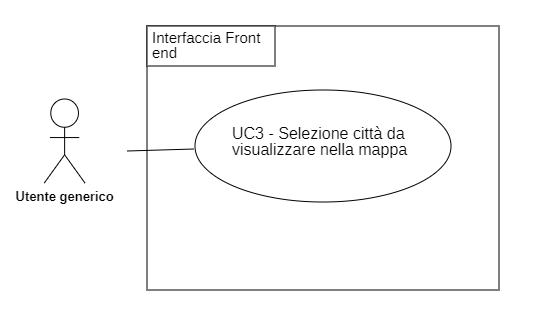
\includegraphics[scale=0.8]{../immagini/attori_casi/uc3.png}
		\caption{UC3 - Zoom della mappa}
	\end{figure}
\end{center}

\begin{itemize}
	\item \textbf{Attori primari:} utente generico;
	\item \textbf{Descrizione:} l’utente, durante la visualizzazione della heat map$_{\scaleto{G}{3pt}}$, può variare il livello di zoom della mappa della città selezionata attraverso l'interfaccia;
	\item \textbf{Scenario principale:} l’utente attraverso l'interfaccia può decidere di:
	\begin{itemize}
		\item aumentare il livello di zoom (UC3.1, sezione \S~\ref{CasiDUsoCasiDUsoTraUnUtenteEIlFrontEndElencoCasiDUsoUC31ZoomInDellaHeatMap});
		\item diminuire il livello di zoom (UC3.2, sezione \S~\ref{CasiDUsoCasiDUsoTraUnUtenteEIlFrontEndElencoCasiDUsoUC32ZoomOutDellaHeatMap}).
	\end{itemize}
	\item \textbf{Precondizione:} il sistema è funzionante e la mappa è stata caricata;
	\item \textbf{Postcondizione:} il livello di zoom della mappa è aumentato o diminuito in base all'azione che compie l'utente: se compie zoom-in il livello aumenta,se invece compie zoom-out il livello diminuisce.
\end{itemize}

\subsubsection{UC3.1 - Zoom-in della heat map}\label{CasiDUsoCasiDUsoTraUnUtenteEIlFrontEndElencoCasiDUsoUC31ZoomInDellaHeatMap}

\begin{center}
	\begin{figure}[H]
		\centering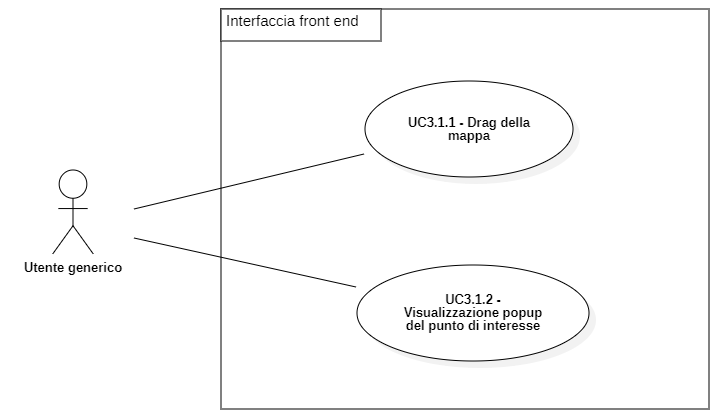
\includegraphics[scale=0.8]{../immagini/attori_casi/uc31_uc32.png}
		\caption{UC3.1 - Zoom-in della heat map}
	\end{figure}
\end{center}

\begin{itemize}
	\item \textbf{Attori primari:} utente generico;
	\item \textbf{Descrizione:} l’utente, durante la visualizzazione della heat map$_{\scaleto{G}{3pt}}$, può aumentare il livello di zoom per vedere in dettaglio la mappa della città selezionata;
	\item \textbf{Scenario principale:} l’utente aumenta il livello di zoom della heat map$_{\scaleto{G}{3pt}}$ per una visualizzazione dettagliata della città, dopo aver compiuto questa azione l'utente inoltre può: spostarsi all'interno della mappa (UC3.1.1, sezione \S~\ref{CasiDUsoCasiDUsoTraUnUtenteEIlFrontEndElencoCasiDUsoUC311DragDellaHeatMap}) e cliccare sui pop-up$_G$ dei punti di interesse (UC3.1.2, sezione \S~\ref{CasiDUsoCasiDUsoTraUnUtenteEIlFrontEndElencoCasiDUsoUC312VisualizzazioneDelPopupDiUnPuntoDiInteresse});
	\item \textbf{Precondizione:} il sistema dispone di informazioni relative alla città e il livello di zoom-in non è al massimo;
	\item \textbf{Postcondizione:} la heat map$_{\scaleto{G}{3pt}}$ si aggiorna mostrando livelli di informazioni più dettagliate in base al livello di zoom in effettuato.
\end{itemize}

\subsubsection{UC3.1.1 - Drag$_G$ della heat map}\label{CasiDUsoCasiDUsoTraUnUtenteEIlFrontEndElencoCasiDUsoUC311DragDellaHeatMap}

\begin{itemize}
	\item \textbf{Attori primari:} utente generico;
	\item \textbf{Descrizione:} l’utente può spostarsi all’interno della heat map$_{\scaleto{G}{3pt}}$;
	\item \textbf{Scenario principale:} l’utente si sposta all’interno della heat map$_{\scaleto{G}{3pt}}$;
	\item \textbf{Precondizione:} il livello di zoom in è diverso da quello iniziale e si sta visualizzando un dettaglio della heat map$_{\scaleto{G}{3pt}}$;
	\item \textbf{Postcondizione:} l’utente si è spostato all’interno della heat map$_{\scaleto{G}{3pt}}$.
\end{itemize}

\subsubsection{UC3.1.2 - Visualizzazione del popup di un punto di interesse}\label{CasiDUsoCasiDUsoTraUnUtenteEIlFrontEndElencoCasiDUsoUC312VisualizzazioneDelPopupDiUnPuntoDiInteresse}

\begin{itemize}
	\item \textbf{Attori primari:} utente generico;
	\item \textbf{Descrizione:} l’utente ha la possibilità di selezionare una zona in particolare della mappa e far apparire un popup contenente le informazioni riguardanti la zona selezionata;	
	\item \textbf{Scenario principale:} l’utente seleziona una zona e appare un popup;
	\item \textbf{Precondizione:} il livello di zoom in è diverso da quello iniziale ed il sistema fa apparire un’icona apposita per il popup;	
	\item \textbf{Postcondizione:} l’utente ha premuto sull’icona ed appare il popup.
\end{itemize}

\subsubsection{UC3.2 - Zoom-out della heat map}\label{CasiDUsoCasiDUsoTraUnUtenteEIlFrontEndElencoCasiDUsoUC32ZoomOutDellaHeatMap}

\begin{itemize}
	\item \textbf{Attori primari:} utente generico;
	\item \textbf{Descrizione:} l’utente, durante la visualizzazione della heat map$_{\scaleto{G}{3pt}}$, può diminuire il livello di zoom per vedere informazioni meno dettagliate della città selezionata;
	\item \textbf{Scenario principale:} l’utente diminuisce il livello di zoom della heat map$_{\scaleto{G}{3pt}}$ per una visualizzazione meno dettagliata della città;
	\item \textbf{Precondizione:}  il sistema dispone di informazioni relative alla città e il livello di zoom-out non è al massimo;
	\item \textbf{Postcondizione:} la heat map$_{\scaleto{G}{3pt}}$ si aggiorna mostrando livelli di informazioni meno dettagliate in base al livello di zoom out effettuato.
\end{itemize}

\subsubsection{UC4 - Selezione città da visualizzare nella mappa}\label{CasiDUsoCasiDUsoTraUnUtenteEIlFrontEndElencoCasiDUsoUC4SelezioneCittaDaVisualizzareNellaMappa} 

\begin{center}
	\begin{figure}[H]
		\centering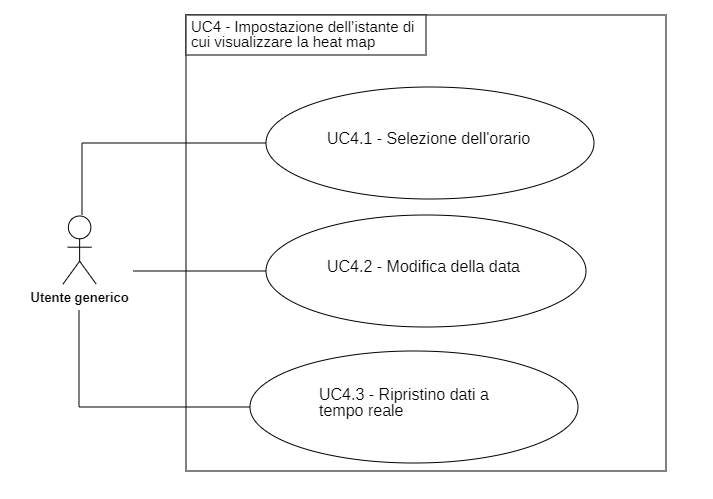
\includegraphics{../immagini/attori_casi/uc4.png}
		\caption{UC4 - Selezione città da visualizzare nella mappa}
	\end{figure}
\end{center}

\begin{itemize}
	\item \textbf{Attori primari}: utente generico;
	\item \textbf{Descrizione}:  l’utente può selezionare la città di cui vuole visualizzare la heat map$_{\scaleto{G}{3pt}}$;
	\item \textbf{Scenario principale}:l’utente seleziona una città tra quelle messe a disposizione;
	\item \textbf{Precondizione}: il sistema dispone di informazioni relative a diverse città;
	\item \textbf{Postcondizione}:   l’utente ha selezionato la città che vuole visualizzare, la heat-map$_{\scaleto{G}{3pt}}$ si aggiorna in base alla scelta fatta.
\end{itemize}

\subsubsection{UC5 - Selezione dell’istante di cui visualizzare i dati nella heat map
}\label{CasiDUsoCasiDUsoTraUnUtenteEIlFrontEndElencoCasiDUsoUC5SelezioneDellIstanzeDiCuiVisualizzareIDatiNellaHeatmap}%parzialmente corretto
\begin{center}
	\begin{figure}[H]
		\centering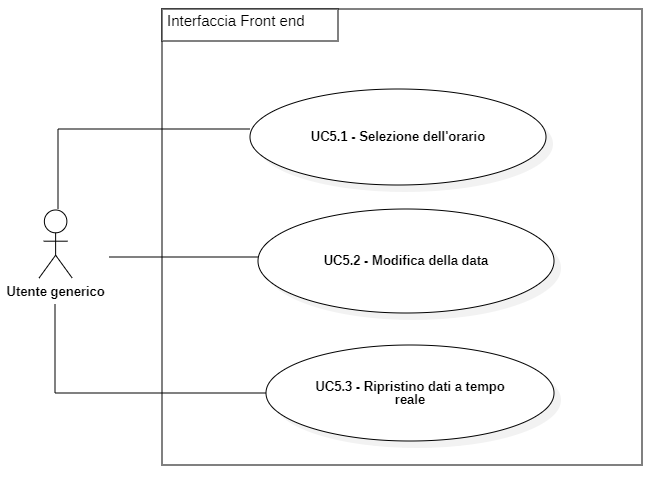
\includegraphics{../immagini/attori_casi/uc5.png}
		\caption{UC5 - Selezione dell’istante di cui visualizzare i dati nella heat map}
	\end{figure}
\end{center}
\begin{itemize}
	\item \textbf{Attori primari}: utente generico;
	\item \textbf{Descrizione}: l’utente, attraverso l’interfaccia del sistema, modifica l’istante di tempo di cui vuole visualizzare i dati;
	\item \textbf{Scenario principale}: attraverso l’interfaccia l’utente può decidere di:
		\begin{enumerate}
			\item Modificare l’orario dei dati da visualizzare (UC5.1, sezione  \S~\ref{CasiDUsoCasiDUsoTraUnUtenteEIlFrontEndElencoCasiDUsoUC51SelezioneDellOrario});
			\item Modificare la data tra quelle disponibili (UC5.2, sezione \S~\ref{CasiDUsoCasiDUsoTraUnUtenteEIlFrontEndElencoCasiDUsoUC52ModificaDellaData});
			\item Ritornare ai dati in tempo reale (UC5.3, sezione \S~\ref{CasiDUsoCasiDUsoTraUnUtenteEIlFrontEndElencoCasiDUsoUC53RipristinoDatiATempoReale}).
		\end{enumerate}
	\item \textbf{Precondizione}: il sistema dispone di informazioni su diversi istanti di tempo;
	\item \textbf{Postcondizione}: l’utente ha selezionato un istante di tempo diverso da quello attuale e visualizza i dati riguardanti ad esso.%insicuro
\end{itemize}

\subsubsection{UC5.1 - Selezione dell’orario}\label{CasiDUsoCasiDUsoTraUnUtenteEIlFrontEndElencoCasiDUsoUC51SelezioneDellOrario}
\begin{itemize}
	\item \textbf{Attori primari}: utente generico;
	\item \textbf{Descrizione}: l’utente seleziona un orario diverso da quello attuale per visualizzare i dati di quel momento;
	\item \textbf{Scenario principale}: l’utente imposta un orario utilizzando l’interfaccia dell’applicazione web;
	\item \textbf{Precondizione}: il sistema ha informazioni riguardanti tutti i diversi orari; %insicuro
	\item \textbf{Postcondizione}:  l’orario viene aggiornato e la mappa visualizza i dati della modifica fatta.
\end{itemize}

\subsubsection{UC5.2 - Modifica della data}\label{CasiDUsoCasiDUsoTraUnUtenteEIlFrontEndElencoCasiDUsoUC52ModificaDellaData}
\begin{itemize}
	\item \textbf{Attori primari}: utente generico;
	\item \textbf{Descrizione}: l’utente seleziona una data diversa da quella odierna tra quelle disponibili e visualizza la mappa della data scelta;
	\item \textbf{Scenario principale}: l’utente seleziona una data diversa da quella attuale;
	\item \textbf{Precondizione}: il sistema possiede informazioni su tutte le date fino a quella odierna;
	\item \textbf{Postcondizione}: la data viene aggiornata e l’utente visualizza l’heat map$_{\scaleto{G}{3pt}}$ aggiornata con i dati del giorno selezionato all’orario attuale o all’orario scelto dall’utente stesso, secondo quanto definito nella descrizione dell’UC5.1 (sezione \S~\ref{CasiDUsoCasiDUsoTraUnUtenteEIlFrontEndElencoCasiDUsoUC51SelezioneDellOrario}).
\end{itemize}

\subsubsection{UC5.3 - Ripristino dati a tempo reale}\label{CasiDUsoCasiDUsoTraUnUtenteEIlFrontEndElencoCasiDUsoUC53RipristinoDatiATempoReale}
\begin{itemize}
	\item \textbf{Attori primari}: utente generico;
	\item \textbf{Descrizione}:  l’utente sceglie di osservare i dati in tempo reale;
	\item \textbf{Scenario principale}: l’utente preme sul pulsante per il ripristino dei valori attuali di data e ora;
	\item \textbf{Precondizione}: l’utente ha impostato una data e/o un’ora diversa dal valore di quella attuale secondo quanto descritto nell'UC5.1 (sezione \S~\ref{CasiDUsoCasiDUsoTraUnUtenteEIlFrontEndElencoCasiDUsoUC51SelezioneDellOrario}) e nell'UC5.2 (sezione \S~\ref{CasiDUsoCasiDUsoTraUnUtenteEIlFrontEndElencoCasiDUsoUC52ModificaDellaData});
	\item \textbf{Postcondizione}: l’utente visualizza la mappa con i dati in tempo reale.
\end{itemize}

\subsubsection{UC6 - Ricerca della città da visualizzare}\label{CasiDUsoCasiDUsoTraUnUtenteEIlFrontEndElencoCasiDUsoUC6RicercaDellaCittàDaVisualizzare}

\begin{center}
	\begin{figure}[H]
		\centering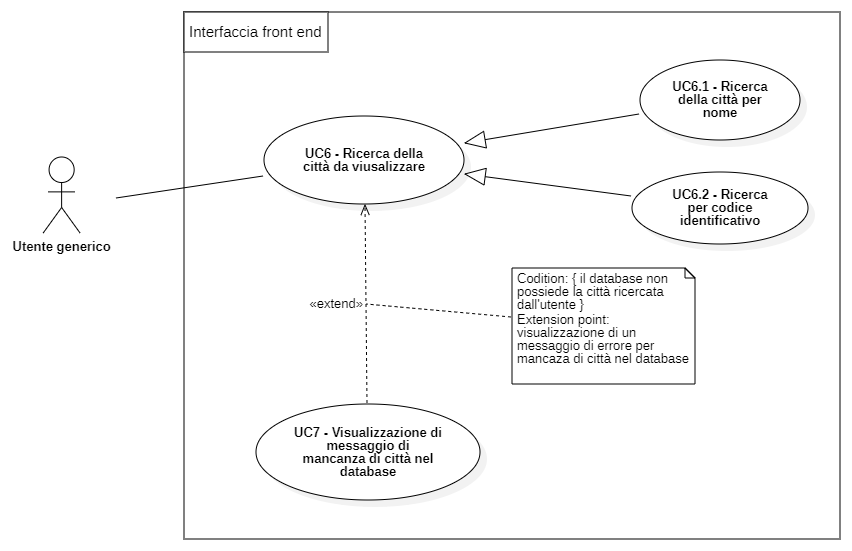
\includegraphics[scale=0.8]{../immagini/attori_casi/uc6.png}
		\caption{UC6 - Ricerca della città da visualizzare}
	\end{figure}
\end{center}

\begin{itemize}
	\item \textbf{Attori primari:} utente generico;
	\item \textbf{Descrizione:} l’utente può ricercare in una barra di ricerca la città da visualizzare;
	\item \textbf{Scenario principale:} l’utente ricerca una città tramite una barra di ricerca;
	\item \textbf{Precondizione:} l’utente ha inserito la città da ricercare;
	\item \textbf{Postcondizione:}l’utente ha inserito la città che vuole cercare e il sistema si aggiorna in base alla ricerca fatta;
	\item \textbf{Estensioni:} l’utente ha ricercato una città non presente nel database, il sistema rileva questo errore e di conseguenza viene visualizzato un messaggio relativo all’errore riscontrato (UC 7, sezione \S~\ref{CasiDUsoCasiDUsoTraUnUtenteEIlFrontEndElencoCasiDUsoUC7VisualizzazioneMessaggioDiMancanzaCittàNelDatabase}).
\end{itemize}

\subsubsection{UC6.1 - Ricerca della città da visualizzare tramite codice identificativo}\label{CasiDUsoCasiDUsoTraUnUtenteEIlFrontEndElencoCasiDUsoUC61RicercaDellaCittàDaVisualizzareTramiteCodiceIdentificativo}

\begin{itemize}
	\item \textbf{Attori primari:} utente generico;
	\item \textbf{Descrizione:} l’utente ha la possibilità di ricercare la città da visualizzare tramite codice identificativo;
	\item \textbf{Scenario principale:} l’utente ricerca la città tramite codice identificativo;
	\item \textbf{Precondizione:} l’utente ha inserito il codice identificativo della città da ricercare;
	\item \textbf{Postcondizione:} il sistema mostra all’utente il risultato della ricerca effettuata.
\end{itemize}

\subsubsection{UC6.2 - Ricerca della città da visualizzare tramite nome}\label{CasiDUsoCasiDUsoTraUnUtenteEIlFrontEndElencoCasiDUsoUC52RicercaDellaCittàDaVisualizzareTramiteNome}

\begin{itemize}
	\item \textbf{Attori primari:} utente generico;
	\item \textbf{Descrizione:} l’utente ha la possibilità di ricercare la città da visualizzare tramite nome;
	\item \textbf{Scenario principale:} l’utente ricerca la città tramite nome;
	\item \textbf{Precondizione:} l’utente ha inserito il nome della città da ricercare;
	\item \textbf{Postcondizione:} il sistema mostra all’utente il risultato della ricerca effettuata.
\end{itemize}

\subsubsection{UC7 - Visualizzazione messaggio di mancanza città nel database}\label{CasiDUsoCasiDUsoTraUnUtenteEIlFrontEndElencoCasiDUsoUC7VisualizzazioneMessaggioDiMancanzaCittàNelDatabase}

\begin{itemize}
	\item \textbf{Attori primari:} utente generico;
	\item \textbf{Descrizione:} l’utente visualizza un messaggio di errore per un inserimento nella barra di ricerca di una città non presente nel database;
	\item \textbf{Scenario principale:} 
	\begin{enumerate}
		\item l’operazione di ricerca fallisce;
		\item l’utente visualizza un messaggio di errore;
		\item l’utente preme "ok" per chiudere il messaggio.
	\end{enumerate}
	\item \textbf{Precondizione:} il front end$_{\scaleto{G}{3pt}}$ effettua un controllo sui dati e non è presente la città ricercata;
	\item \textbf{Postcondizione:} viene visualizzato  un messaggio all’utente per informarlo sul problema.
\end{itemize}

\section{Casi d'uso tra il front end e il back end}\label{CasiDUsoCasiDUsoTraIlFrontEndEIlBackEnd}
%spiegazione sezione

\subsection{Attori dei casi d'uso}\label{CasiDUsoCasiDUsoTraIlFrontEndEIlBackEndAttoriDeiCasiDUso}
%immagine errata
\begin{center}
	\begin{figure}[H]
		\centering
\includegraphics{../immagini/attori_casi/sistema_front_end.png}
		\caption{Attore: Sistema front end}
	\end{figure}
\end{center}
\subsubsection{Attori Primari}\label{CasiDUsoCasiDUsoTraIlFrontEndEIlBackEndAttoriDeiCasiDUsoAttoriPrimari}
\begin{itemize}
	\item \textbf{Sistema front end$_{\scaleto{G}{3pt}}$:} Definisce una parte del sistema sviluppato che interagisce con il sistema back end$_{\scaleto{G}{3pt}}$;
\end{itemize}

\subsection{Elenco casi d'uso}\label{CasiDUsoCasiDUsoTraIlFrontEndEIlBackEndElencoDeiCasiDUso}


\subsubsection{UC8 - Visualizzazione delle informazioni dal back end}\label{CasiDUsoCasiDUsoTraIlFrontEndEIlBackEndElencoDeiCasiDUsoUC8VisualizzazioneDelleInformazioniDalBackEnd}
\begin{center}
	\begin{figure}[H]
		\centering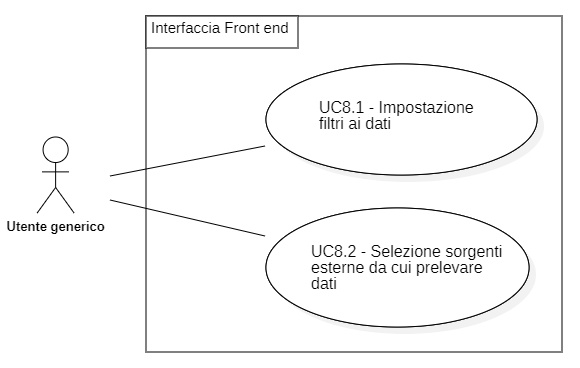
\includegraphics[scale=0.7]{../immagini/attori_casi/uc8.png}
		\caption{UC8 - Visualizzazione delle informazioni dal back end}
	\end{figure}
\end{center}
\begin{itemize}
	\item \textbf{Attori primari}: sistema front end$_{\scaleto{G}{3pt}}$;
	\item \textbf{Descrizione}: il front end$_{\scaleto{G}{3pt}}$ effettua una richiesta per il recupero dei dati al back end$_{\scaleto{G}{3pt}}$ per generare la heat-map$_{\scaleto{G}{3pt}}$. Il back end$_{\scaleto{G}{3pt}}$ esegue a richiesta ed invia le informazioni da visualizzare al front end$_{\scaleto{G}{3pt}}$;
	\item \textbf{Scenario principale}: il front end$_{\scaleto{G}{3pt}}$ richiede al back end$_{\scaleto{G}{3pt}}$ le informazioni necessarie alla generazione della heat map$_{\scaleto{G}{3pt}}$, il front end$_{\scaleto{G}{3pt}}$ visualizza le informazioni ricevute dal back end$_{\scaleto{G}{3pt}}$;
	\item \textbf{Precondizione}: il front end$_{\scaleto{G}{3pt}}$ non ha le informazioni per poter generare la mappa;
	\item \textbf{Postcondizione}: il front end$_{\scaleto{G}{3pt}}$ visualizza e riceve le nuove informazioni. 
	\item \textbf{Generalizzazioni}: il front end$_{\scaleto{G}{3pt}}$ può fare una delle seguenti richieste:
	\begin{itemize}
		\item Visualizza i dati di uno specifico istante (UC8.1, sezione \S~\ref{CasiDUsoCasiDUsoTraIlFrontEndEIlBackEndElencoDeiCasiDUsoUC81VisualizzazioneDeiDatiDiUnoSpecificoIstante});
		\item Visualizza i dati in tempo reale (UC8.2, sezione  \S~\ref{CasiDUsoCasiDUsoTraIlFrontEndEIlBackEndElencoDeiCasiDUsoUC82VisualizzazioneDeiDatiInTempoReale});
		\item Visualizza i dati predetti (UC8.3, sezione  \S~\ref{CasiDUsoCasiDUsoTraIlFrontEndEIlBackEndElencoDeiCasiDUsoUC83VisualizzazioneDeiDatiPredetti}).
	\end{itemize}
	\item \textbf{Estensione}: il front end$_{\scaleto{G}{3pt}}$ effettua la richiesta al back end$_{\scaleto{G}{3pt}}$ il quale non invia nessun dato nella risposta (UC9, sezione \S~\ref{CasiDUsoCasiDUsoTraIlFrontEndEIlBackEndElencoDeiCasiDUsoUC9VisualizzazioneMessaggioDiMancanzaDatiDalBackEnd}).
\end{itemize}

\subsubsection{UC8.1 - Visualizzazione dei dati di uno specifico istante}\label{CasiDUsoCasiDUsoTraIlFrontEndEIlBackEndElencoDeiCasiDUsoUC81VisualizzazioneDeiDatiDiUnoSpecificoIstante}
\begin{itemize}
	\item \textbf{Attori primari}: sistema front end$_{\scaleto{G}{3pt}}$;
	\item \textbf{Descrizione}: il front end$_{\scaleto{G}{3pt}}$ richiede le informazioni relative ad uno specifico istante di tempo, vengono visualizzate le informazioni inviate dal back end$_{\scaleto{G}{3pt}}$;
	\item \textbf{Scenario principale}:  il front end$_{\scaleto{G}{3pt}}$ richiede al back end$_{\scaleto{G}{3pt}}$ le informazioni relative all'istante di tempo specificato, il back end$_{\scaleto{G}{3pt}}$ invia le informazioni da visualizzare al front end$_{\scaleto{G}{3pt}}$;
	\item \textbf{Precondizione}: l’utente esegue la modifica della data o dell’orario come definito rispettivamente nella descrizione di UC5.2 (sezione \S~\ref{CasiDUsoCasiDUsoTraUnUtenteEIlFrontEndElencoCasiDUsoUC52ModificaDellaData}) e UC5.1 (sezione \S~\ref{CasiDUsoCasiDUsoTraUnUtenteEIlFrontEndElencoCasiDUsoUC51SelezioneDellOrario}) selezionando un istante di tempo precedente a quello attuale;
	\item \textbf{Postcondizione}: il front end$_{\scaleto{G}{3pt}}$ visualizza e riceve le informazioni relative all'istante di tempo impostato. 
\end{itemize}

\subsubsection{UC8.2 - Visualizzazione dei dati in tempo reale}\label{CasiDUsoCasiDUsoTraIlFrontEndEIlBackEndElencoDeiCasiDUsoUC82VisualizzazioneDeiDatiInTempoReale}
\begin{itemize}
	\item \textbf{Attori primari}: sistema front end$_{\scaleto{G}{3pt}}$;
	\item \textbf{Descrizione}: il front end$_{\scaleto{G}{3pt}}$ visualizza i dati reali più recentemente aggiunti;
	\item \textbf{Scenario principale}: il front end$_{\scaleto{G}{3pt}}$ richiede al back end$_{\scaleto{G}{3pt}}$ le informazioni più recentemente aggiunte, una volta ricevute il front end$_{\scaleto{G}{3pt}}$ le visualizza;
	\item \textbf{Precondizione}: viene eseguita la visualizzazione della mappa come definito nell’UC1 (sezione \S~\ref{CasiDUsoCasiDUsoTraUnUtenteEIlFrontEndElencoCasiDUsoUC1VisualizzazioneInformazioniSullaMappa}) o avviene il ripristino dei dati in tempo reale come definito in UC5.3 (sezione \S~\ref{CasiDUsoCasiDUsoTraUnUtenteEIlFrontEndElencoCasiDUsoUC53RipristinoDatiATempoReale});
	\item \textbf{Postcondizione}: il front end$_{\scaleto{G}{3pt}}$ ha ricevuto e visualizzato i dati ed è pronto alla generazione della heat map$_{\scaleto{G}{3pt}}$. 
\end{itemize}

\subsubsection{UC8.3 - Visualizzazione dei dati predetti}\label{CasiDUsoCasiDUsoTraIlFrontEndEIlBackEndElencoDeiCasiDUsoUC83VisualizzazioneDeiDatiPredetti}
\begin{itemize}
	\item \textbf{Attori primari}: sistema front end$_{\scaleto{G}{3pt}}$;
	\item \textbf{Descrizione}: il front end$_{\scaleto{G}{3pt}}$ richiede i dati riferiti allo stesso giorno, ma ad un orario avanzato rispetto a quello attuale.
	I dati sono ricavati dall’elaborazione, attraverso un modello di machine learning$_{\scaleto{G}{3pt}}$, dei dati reali acquisti. Una volta ricevuti i dati il front end$_{\scaleto{G}{3pt}}$ li può visualizzare;
	\item \textbf{Scenario principale}: il front end$_{\scaleto{G}{3pt}}$ richiede al back end$_{\scaleto{G}{3pt}}$ i dati elaborati dal modello machine learning$_{\scaleto{G}{3pt}}$. Completata la richiesta il front end$_{\scaleto{G}{3pt}}$ visualizzerà i dati inviati dal back end$_{\scaleto{G}{3pt}}$;
	\item \textbf{Precondizione}: le informazioni vengono visualizzate sulla mappa come definito nell’UC1 (sezione \S~\ref{CasiDUsoCasiDUsoTraUnUtenteEIlFrontEndElencoCasiDUsoUC1VisualizzazioneInformazioniSullaMappa}), impostando un orario successivo a quello attuale come descritto nell’UC5.1 (sezione \S~\ref{CasiDUsoCasiDUsoTraUnUtenteEIlFrontEndElencoCasiDUsoUC51SelezioneDellOrario});
	\item \textbf{Postcondizione}: il front end$_{\scaleto{G}{3pt}}$ ha ricevuto e visualizzato i dati ed è pronto alla generazione della heat map$_{\scaleto{G}{3pt}}$. 
\end{itemize}

\subsubsection{UC9 - Visualizzazione messaggio di mancanza dati dal back end}\label{CasiDUsoCasiDUsoTraIlFrontEndEIlBackEndElencoDeiCasiDUsoUC9VisualizzazioneMessaggioDiMancanzaDatiDalBackEnd}
\begin{itemize}
	\item \textbf{Attori primari}: sistema front end$_{\scaleto{G}{3pt}}$;
	\item \textbf{Descrizione}: il front end$_{\scaleto{G}{3pt}}$ riceve un messaggio di errore per la mancanza dati rispetto alla richiesta di visualizzazione effettuata;
	\item \textbf{Scenario principale}: 
	\begin{enumerate}
		\item Il front end$_{\scaleto{G}{3pt}}$ richiede dei dati specifici al back end$_{\scaleto{G}{3pt}}$;
		\item La risposta ricevuta è un messaggio di errore;
		\item Il front end$_{\scaleto{G}{3pt}}$ ritenta la richiesta di informazioni. 
	\end{enumerate}
	\item \textbf{Precondizione}: il front end$_{\scaleto{G}{3pt}}$ effettua una richiesta di dati, il back end$_{\scaleto{G}{3pt}}$ non ha a disposizione i dati richiesti;
	\item \textbf{Postcondizione}: il front end$_{\scaleto{G}{3pt}}$ riceve un messaggio di errore per la mancanza dei dati da visualizzare. 
\end{itemize}

\newpage
\section{Casi d'uso facoltativi tra un utente e il front end}\label{CasiDUsoCasiDUsoFacoltativiTraUnUtenteEIlFrontEnd}
%spiegazione della sezione
L'elenco dei casi d'uso in questa sezione individuano requisiti sviluppabili successivamente a quelli obbligatori descritti nelle sezioni precedenti.
\subsection{Attori dei casi d'uso}
\begin{center}
	\begin{figure}[H]
		\centering
\includegraphics{../immagini/attori_casi/utente_generico.png}
		\caption{Attore: utente generico}
	\end{figure}
\end{center}
\subsubsection{Attori Primari}\label{UFattoriPrimariFac}
\begin{itemize}
	\item \textbf{Utente generico:} definisce l'utente generico che utilizza l'applicazione web;
\end{itemize}

\subsection{Elenco casi d'uso}\label{CasiDUsoCasiDUsoFacoltativiTraUnUtenteEIlFrontEndElencoCasiDUso}

\subsubsection{UC10 - Visualizzazione indici di affidabilità}\label{CasiDUsoCasiDUsoFacoltativiTraUnUtenteEIlFrontEndElencoCasiDUsoUC10VisualizzazioneIndiciDiAffidabilita}

\begin{center}
	\begin{figure}[H]
		\centering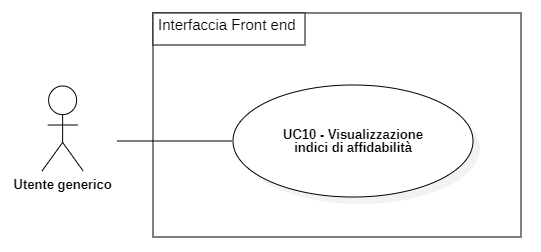
\includegraphics[scale=0.7]{../immagini/attori_casi/uc10.png}
		\caption{UC10 - Visualizzazione indici di affidabilità}
	\end{figure}
\end{center}

\begin{itemize}
	\item \textbf{Attori primari}: utente generico;
	\item \textbf{Descrizione}: l'utente può visualizzare gli indici di affidabilità dei dati reali raccolti e l'indice di affidabilità delle predizioni svolte dal modello di machine learning$_{\scaleto{G}{3pt}}$;
	\item \textbf{Scenario principale}: l'utente attraverso l'interfaccia seleziona un pulsante per visualizzare gli indici di affidabilità;
	\item \textbf{Precondizione}: il front end$_{\scaleto{G}{3pt}}$ dispone degli indici relativi ai dati reali e predetti;
	\item \textbf{Postcondizione}: l'utente visualizza correttamente gli indici di affidabilità dei dati reali e predetti. 
\end{itemize}

\subsubsection{UC11 - Impostazioni avanzate sui dati}\label{CasiDUsoCasiDUsoFacoltativiTraUnUtenteEIlFrontEndElencoCasiDUsoUC11ImpostazioniAvanzateSuiDati}

\begin{center}
	\begin{figure}[H]
		\centering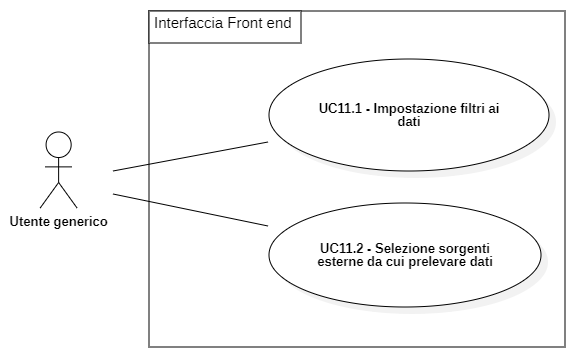
\includegraphics[scale=0.7]{../immagini/attori_casi/uc11.png}
		\caption{UC11 - Impostazioni avanzate sui dati}
	\end{figure}
\end{center}

\begin{itemize}
	\item \textbf{Attori primari}: utente generico;
	\item \textbf{Descrizione}: l'utente attraverso l'interfaccia del front end$_{\scaleto{G}{3pt}}$ può applicare filtri sui dati e modificare le sorgenti esterne da cui vengono prelevate le informazioni;
	\item \textbf{Scenario principale}: attraverso l'interfaccia l'utente può:
	\begin{itemize}
		\item Applicare filtri ai dati (UC11.1, sezione  \S~\ref{CasiDUsoCasiDUsoFacoltativiTraUnUtenteEIlFrontEndElencoCasiDUsoUC111ApplicazioneFiltriAiDati});
		\item Modificare le sorgenti esterne da cui vengono prelevate le informazioni (UC11.2, sezione \S~\ref{CasiDUsoCasiDUsoFacoltativiTraUnUtenteEIlFrontEndElencoCasiDUsoUC112SelezioneSorgentiEsterneDaCuiPrelevareIDati});
	\end{itemize}
	\item \textbf{Precondizione}: l'utente visualizza correttamente l'interfaccia e sono disponibili varie sorgenti esterne;
	\item \textbf{Postcondizione}: l'utente applica le impostazioni scelte ai dati e viene aggiornata la mappa di conseguenza. 
\end{itemize}

\subsubsection{UC11.1 - Applicazione filtri ai dati}\label{CasiDUsoCasiDUsoFacoltativiTraUnUtenteEIlFrontEndElencoCasiDUsoUC111ApplicazioneFiltriAiDati}
\begin{itemize}
	\item \textbf{Attori primari}: utente generico;
	\item \textbf{Descrizione}: l'utente attraverso l'interfaccia del front end$_{\scaleto{G}{3pt}}$ può applicare filtri sui dati reali e su quelli predetti, modificandone i colori con cui vengono visualizzati nella mappa;
	\item \textbf{Scenario principale}: 
	\begin{enumerate}
		\item L'utente può selezionare il colore per i dati reali e/o per quelli predetti;
		\item L'utente conferma i filtri da applicare alla mappa. 
	\end{enumerate}
	\item \textbf{Precondizione}: l'utente visualizza correttamente l'interfaccia;
	\item \textbf{Postcondizione}: l'utente applica i filtri ai dati e viene aggiornata la mappa di conseguenza. 
\end{itemize}

\subsubsection{UC11.2 - Selezione sorgenti esterne da cui prelevare i dati}\label{CasiDUsoCasiDUsoFacoltativiTraUnUtenteEIlFrontEndElencoCasiDUsoUC112SelezioneSorgentiEsterneDaCuiPrelevareIDati}
\begin{itemize}
	\item \textbf{Attori primari}: utente generico;
	\item \textbf{Descrizione}: l'utente attraverso l'interfaccia del front end$_{\scaleto{G}{3pt}}$ dispone di un menù in cui può selezionare le sorgenti che vuole utilizzare per il reperimento dei dati;
	\item \textbf{Scenario principale}: l'utente seleziona la modifica delle sorgenti esterne e indica quelle da cui vuole prelevare informazioni;
	\item \textbf{Precondizione}: l'utente visualizza correttamente l'interfaccia, sono disponibili varie sorgenti esterne;
	\item \textbf{Postcondizione}: l'utente visualizza la mappa con i soli dati delle sorgenti scelte. 
\end{itemize}

\subsubsection{UC12 - Recupero manuale utente}\label{CasiDUsoCasiDUsoFacoltativiTraUnUtenteEIlFrontEndElencoCasiDUsoUC12RecuperoManualeUtente}

\begin{center}
	\begin{figure}[H]
		\centering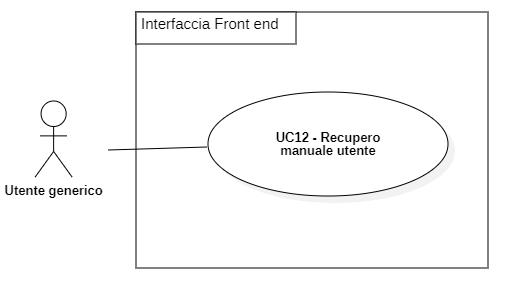
\includegraphics[scale=0.7]{../immagini/attori_casi/uc12.png}
		\caption{UC12 - Recupero manuale utente}
	\end{figure}
\end{center}

\begin{itemize}
	\item \textbf{Attori primari}: utente generico;
	\item \textbf{Descrizione}: l'utente attraverso l'interfaccia del front end$_{\scaleto{G}{3pt}}$ può recuperare il manuale d'uso per informazioni sull'utilizzo dell'applicazione web;
	\item \textbf{Scenario principale}: l'utente seleziona il link al recupero del manuale utente;
	\item \textbf{Precondizione}: il front end$_{\scaleto{G}{3pt}}$ dispone del manuale utente;
	\item \textbf{Postcondizione}: l'utente dispone del manuale utente sul proprio dispositivo e lo può visualizzare. 
\end{itemize}

\subsubsection{UC13 -Visualizzazione di dati a confronto di due città differenti}\label{CasiDUsoCasiDUsoFacoltativiTraUnUtenteEIlFrontEndElencoCasiDUsoUC13VisualizzazioneDiDatiAConfrontoDiDueCittaDifferenti}

\begin{center}
	\begin{figure}[H]
		\centering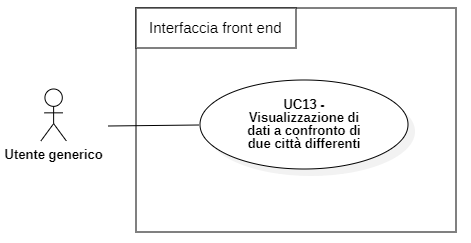
\includegraphics[scale=0.7]{../immagini/attori_casi/uc13.png}
		\caption{UC13 - Visualizzazione di dati a confronto di due città differenti}
	\end{figure}
\end{center}

\begin{itemize}
	\item \textbf{Attori primari}: utente generico;
	\item \textbf{Descrizione}: l’utente può selezionare due città per poter mettere a confronto i loro dati;
	\item \textbf{Scenario principale}: l’utente seleziona le due città;
	\item \textbf{Precondizione}: il sistema dispone le informazioni riguardanti le città;
	\item \textbf{Postcondizione}: l'utente visualizza i dati di entrambe le città per poterli mettere a confronto. 
\end{itemize}

\subsubsection{UC14 -Salvataggio dei dati di una città in un file esterno}\label{CasiDUsoCasiDUsoFacoltativiTraUnUtenteEIlFrontEndElencoCasiDUsoUC14SalvataggioDeiDatiDiUnaCittaInUnFileEsterno}

\begin{center}
	\begin{figure}[H]
		\centering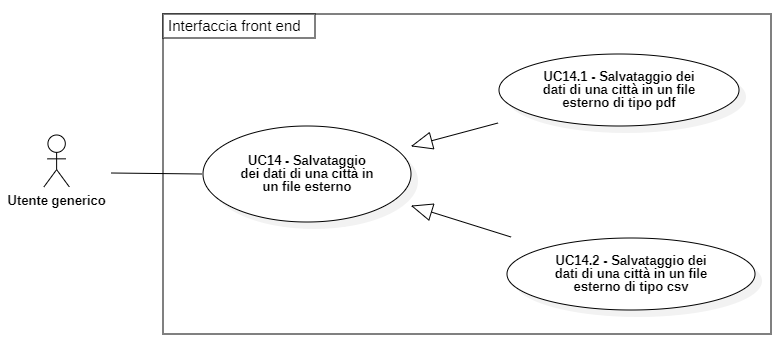
\includegraphics[scale=0.7]{../immagini/attori_casi/uc14.png}
		\caption{UC14 - Salvataggio dei dati di una città in un file esterno}
	\end{figure}
\end{center}

\begin{itemize}
	\item \textbf{Attori primari}: utente generico;
	\item \textbf{Descrizione}: l’utente ha la possibilità di salvare localmente i dati relativi ad una città in un file;
	\item \textbf{Scenario principale}: l’utente salva localmente i dati della città che sta visualizzando;
	\item \textbf{Precondizione}: il sistema dispone le informazioni riguardanti le città e  l’utente sta visualizzando la heat map$_{\scaleto{G}{3pt}}$ di una città in particolare;
	\item \textbf{Postcondizione}: il sistema ha salvato localmente i dati della città che sta visualizzando. 
\end{itemize}

\subsubsection{UC14.1 -Salvataggio dei dati di una città in un file esterno di tipo pdf}\label{CasiDUsoCasiDUsoFacoltativiTraUnUtenteEIlFrontEndElencoCasiDUsoUC141SalvataggioDeiDatiDiUnaCittaInUnFileEsternoDiTipoPdf}

\begin{itemize}
	\item \textbf{Attori primari}: utente generico;
	\item \textbf{Descrizione}: l’utente può selezionare l’estensione del file in pdf;
	\item \textbf{Scenario principale}: l’utente seleziona l’estensione del file in pdf;
	\item \textbf{Precondizione}: il sistema dispone le informazioni riguardanti le città e  l’utente sta visualizzando la heat map$_{\scaleto{G}{3pt}}$ di una città in particolare;
	\item \textbf{Postcondizione}: il sistema ha salvato localmente i dati in formato pdf.
\end{itemize}

\subsubsection{UC14.2 -Salvataggio dei dati di una città in un file esterno di tipo csv}\label{CasiDUsoCasiDUsoFacoltativiTraUnUtenteEIlFrontEndElencoCasiDUsoUC142SalvataggioDeiDatiDiUnaCittaInUnFileEsternoDiTipoCsv}

\begin{itemize}
	\item \textbf{Attori primari}: utente generico;
	\item \textbf{Descrizione}: l’utente può selezionare l’estensione del file in csv;
	\item \textbf{Scenario principale}: l’utente seleziona l’estensione del file in csv;
	\item \textbf{Precondizione}: il sistema dispone le informazioni riguardanti le città e  l’utente sta visualizzando la heat map$_{\scaleto{G}{3pt}}$ di una città in particolare;
	\item \textbf{Postcondizione}: il sistema ha salvato localmente i dati in formato csv.
\end{itemize}

\subsubsection{UC15 - Notifica via email di una città selezionata}\label{CasiDUsoCasiDUsoFacoltativiTraUnUtenteEIlFrontEndElencoCasiDUsoUC15NotificaViaEmailDiUnaCittaSelezionata}

\begin{center}
	\begin{figure}[H]
		\centering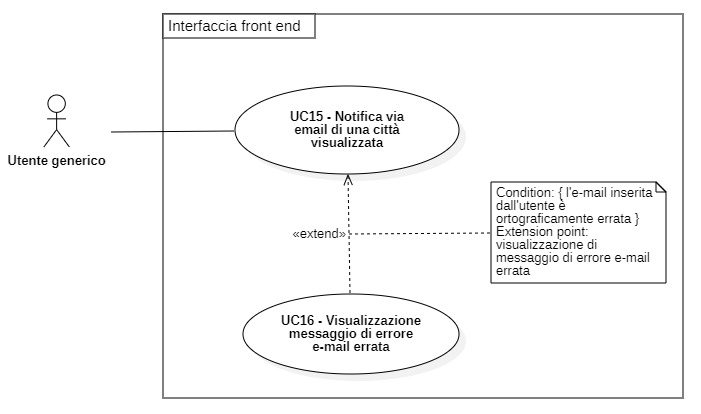
\includegraphics[scale=0.7]{../immagini/attori_casi/uc15.png}
		\caption{UC15 - Notifica via email di una città selezionata}
	\end{figure}
\end{center}

\begin{itemize}
	\item \textbf{Attori primari}: utente generico;
	\item \textbf{Descrizione}: l'utente ha la possibilità di richiedere una notifica via email che verrà inviata nel momento in cui il rischio di assembramento, nella città che sta visualizzando, supera una certa soglia. Per procedere con la richiesta di notifica l'utente deve completare il form di inserimento dell'email;
	\item \textbf{Scenario principale}: l'utente richiede la notifica via email inserendola nel form;
	\item \textbf{Precondizione}: l'utente sta visualizzando la heat map$_{\scaleto{G}{3pt}}$ e richiede la notifica via email;
	\item \textbf{Postcondizione}: il sistema aggiunge nel database l'email inserita dall'utente;
	\item \textbf{Estensioni}: il front end effettua un controllo ortografico che segnala possibili errori all'utente (UC16, sezione \S~\ref{CasiDUsoCasiDUsoFacoltativiTraUnUtenteEIlFrontEndElencoCasiDUsoUC16VisualizzazioneMessaggioDiErroreEmailErrata}).
\end{itemize}

\subsubsection{UC16 - Visualizzazione messaggio di errore e-mail errata}\label{CasiDUsoCasiDUsoFacoltativiTraUnUtenteEIlFrontEndElencoCasiDUsoUC16VisualizzazioneMessaggioDiErroreEmailErrata}

\begin{itemize}
	\item \textbf{Attori primari}: utente generico;
	\item \textbf{Descrizione}: Il front end$_{\scaleto{G}{3pt}}$ invia un messaggio di errore per un inserimento ortografico errato;
	\item \textbf{Scenario principale}: l'utente legge il messaggio inviato dal front end e capisce che deve controllare l'email inserita;
	\item \textbf{Precondizione}: il front end$_{\scaleto{G}{3pt}}$ blocca l'invio di dati al database;
	\item \textbf{Postcondizione}: il front end$_{\scaleto{G}{3pt}}$ invia un messaggio di errore.
\end{itemize}

\subsubsection{UC17 - Visualizzazione lista delle città più cercate}\label{CasiDUsoCasiDUsoFacoltativiTraUnUtenteEIlFrontEndElencoCasiDUsoUC17VisualizzazioneListaDelleCittaPiuCercate}

\begin{center}
	\begin{figure}[H]
		\centering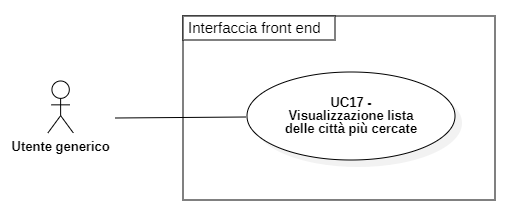
\includegraphics[scale=0.7]{../immagini/attori_casi/uc17.png}
		\caption{UC17 - Visualizzazione lista delle città più cercate}
	\end{figure}
\end{center}

\begin{itemize}
	\item \textbf{Attori primari}: utente generico;
	\item \textbf{Descrizione}: l'utente ha la possibilità di visionare la lista delle città più cercate all'interno del sito; 
	\item \textbf{Scenario principale}: l'utente visualizza la lista;
	\item \textbf{Precondizione}: il sistema è funzionante e possiede le informazioni riguardanti alle ricerche effettuate dagli utenti;
	\item \textbf{Postcondizione}: il back end$_{\scaleto{G}{3pt}}$ invia al front end$_{\scaleto{G}{3pt}}$ la lista delle città più cercate che verrà visualizzata dall'utente.
\end{itemize}

\subsubsection{UC18 - Visualizzazione lista delle città presenti in ordine crescente per rischio}\label{CasiDUsoCasiDUsoFacoltativiTraUnUtenteEIlFrontEndElencoCasiDUsoUC18VisualizzazioneListaDelleCittaPresentiInOrdineCrescentePerRischio}

\begin{center}
	\begin{figure}[H]
		\centering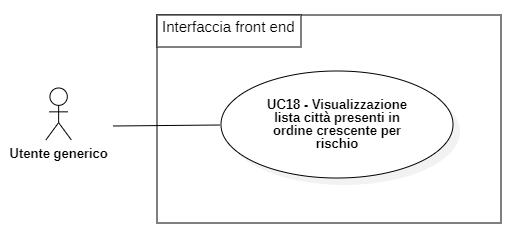
\includegraphics[scale=0.7]{../immagini/attori_casi/uc18.png}
		\caption{UC18 - Visualizzazione lista delle città presenti in ordine crescente per rischio}
	\end{figure}
\end{center}

\begin{itemize}
	\item \textbf{Attori primari}: utente generico;
	\item \textbf{Descrizione}: l'utente ha la possibilità di visionare la lista delle città presenti nel sito in ordine crescente per rischio; 
	\item \textbf{Scenario principale}: l'utente visualizza la lista;
	\item \textbf{Precondizione}:  il sistema è funzionante e possiede le informazioni riguardanti le città;
	\item \textbf{Postcondizione}: il back end$_{\scaleto{G}{3pt}}$ invia al front end$_{\scaleto{G}{3pt}}$ la lista delle città in ordine crescente per rischio che verrà visualizzata dall'utente.
\end{itemize}